%Included libraries
\documentclass[landscape,twocolum,letterpaper]{article}
\usepackage{graphicx}
\usepackage[margin=1.4cm]{geometry}
\usepackage{paralist}
%\usepackage{chemformula}
\setlength{\columnseprule}{0.8pt}
\usepackage{soul,color}
\usepackage{multicol}
\usepackage{caption}
\usepackage{tabularx}
\usepackage{booktabs}
\usepackage[document]{ragged2e}
\usepackage{gensymb}
\usepackage{color, colortbl}
\definecolor{Gray}{gray}{0.9}
\newenvironment{Figure}
	{\par\medskip\noindent\minipage{\linewidth}}
		{\endminipage\par\medskip}
\usepackage{lipsum}
\usepackage{tikz}
\usetikzlibrary{shapes.geometric, arrows}
\newcommand\tab[1][1cm]{\hspace*{#1}}
\usepackage{tikz}
\usepackage{pagecolor}
%flow chart declarations
\tikzstyle{box} = [rectangle, rounded corners, minimum width = 1cm, minimum height=1cm,text justified, text width=8cm, draw=black, fill=white]
\tikzstyle{dat} = [rectangle, rounded corners, minimum width = 0.5cm, minimum height=0.5cm, text centered, draw=black, fill=red!40]
\tikzstyle{bar} = [rectangle, minimum width=30cm, minimum height=1cm, draw=white, fill=purple!50!blue]
\tikzstyle{dia} = [diamond, minimum width=1cm, minimum height=0.4cm, text centered, draw=black, fill=green!30]
\tikzstyle{arrow} = [thick,->,>=stealth]
%Title and authors
\begin{document}
%need to include the Clemson Seal somewhere.
\center
\fontsize{18}{18}\selectfont{\textbf{Widespread Genotype-Phenotype Correlations in Intellectual Disability Associated with Specific Comorbidities and Secondary Clinical Phenotypes}}\\
\fontsize{8}{8}\selectfont{Zachary Gerstner$^1$, Emily L. Casanova$^{2,3}$, Julia L. Sharp$^4$, Manuel F. Casanova$^{2,3}$, Alex Feltus$^1$}\\
\centering
\begin{compactenum}
	\item Department of Genetics and Biochemistry, Clemson University, Clemson, South Carolina, USA
	\item Department of Biomedical Sciences, University of South Carolina Medical School at Greenville, South Carolina, USA
	\item Department of Pediatrics, Greenville Health System, Greenville, South Carolina, USA
	\item Department of Statistics, Colorado State University, Fort Collins, Colorado, USA
\end{compactenum}
%Goals

\begin{tikzpicture}
\node (start) [bar] {};
\end{tikzpicture}
\begin{multicols*}{3}
\flushleft
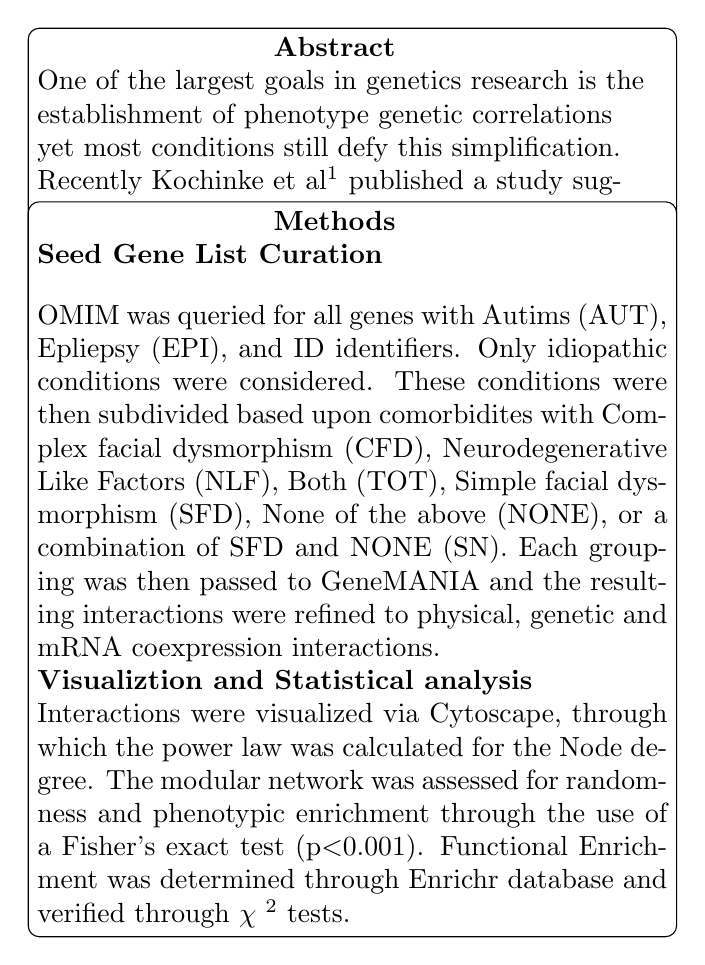
\begin{tikzpicture}[node distance=4.7cm]
\node (start) [box] {\tab \tab \tab \selectfont{\textbf{Abstract}} \\ One of the largest goals in genetics research is the establishment of phenotype genetic correlations yet most conditions still defy this simplification. Recently Kochinke et al$^1$ published a study suggesting that such correlations can be established for Intellectual Disorders (IDs). Our study expands upon their work and identifies distinctive genetic modules whose functional enrichments reflect the clinical phenotypes.};
\node (n1) [box, below of=start] {\tab \tab \tab \selectfont{\textbf{Methods}} \\ \textbf{Seed Gene List Curation}\\ \justify OMIM was queried for all genes with Autims (AUT), Epliepsy (EPI), and ID identifiers. Only idiopathic conditions were considered. These conditions were then subdivided based upon comorbidites with Complex facial dysmorphism (CFD), Neurodegenerative Like Factors (NLF), Both (TOT), Simple facial dysmorphism (SFD), None of the above (NONE), or a combination of SFD and NONE (SN). Each grouping was then passed to GeneMANIA and the resulting interactions were refined to physical, genetic and mRNA coexpression interactions.\\ \textbf{Visualiztion and Statistical analysis}\\ Interactions were visualized via Cytoscape, through which the power law was calculated for the Node degree. The modular network was assessed for randomness and phenotypic enrichment through the use of a Fisher's exact test (p$<$0.001). Functional Enrichment was determined through Enrichr database and verified through $\chi$ $^2$ tests.};
\end{tikzpicture}
\justify
%Gene curation
%\fontsize{12}{12}\selectfont{\textbf{Methods}}
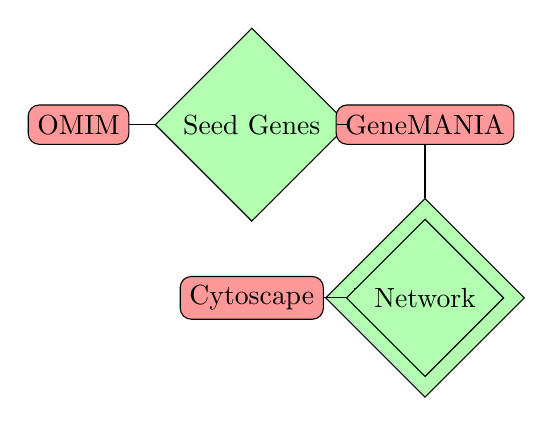
\begin{tikzpicture}[node distance=2.2cm]
\node (start) [dat] {OMIM};
\node (next1) [dia, right of=start] {Seed Genes};
\node (next2) [dat, right of=next1] {GeneMANIA};
\node (next3) [dia, below of=next2] {Interactions};
\node (next4) [dat, left of=next3] {Cytoscape};
\node (stop) [dia, right of=next4] {Network};
\draw (start)--(next1);
\draw (next1)--(next2);
\draw (next2)--(next3);
\draw (next3)--(next4);
\draw (next4)--(stop);
\end{tikzpicture}\\
\fontsize{7}{7}\selectfont{Figure 1. Workflow of the Interaction network generation. Beginning with OMIM query and ending with visualiztion via cytoscape.}\\ \\  
%\columnbreak

%Main Figure
\centering
\fontsize{9}{9}\selectfont{\textbf{Results}}\\
\begin{Figure}
		\includegraphics[width=\columnwidth]{/home/zigerst/Downloads/cas-1.jpeg}
		\justify
		\fontsize{7}{7}\selectfont{Figure 2. Gene interaction network of all IDs.A) Network Overview. B) MECP2 and FMR1 cluster linkages. C) CPSF1 cluster linkage. D) PPT1 cluster linkage E) PRPF8 cluster linkage}
\end{Figure}
\justify

\begin{tabular}{m{2cm}m{2cm}m{2.8cm}}
\toprule
AUT/CFD & EPI/CFD & EPI/NLF\\ \midrule
\rowcolor{Gray}
chromatin modification & histone modification & myelin sheath\\
histone modification & mRNA processing & polyadenylation\\
\rowcolor{Gray}
methylation & Spliceosomal complex & carboxylic acid biosynthetic process\\
transcription factor binding & kinase binding & protein folding\\
\rowcolor{Gray}
 & chromatin binding & \\
\hline
\end{tabular}
\fontsize{8}{8}\selectfont{Table 3. Functional enrichment for Autism and Epilepsy groups. Most groups showed minimal functional enrichment trends.}\\ \\

\begin{Figure}
        \includegraphics[width=\columnwidth]{/home/zigerst/Downloads/CLUSTER.jpg}
        \centering
        \captionof{figure}{Phenotypic enrichment of MCL clusters.}
\end{Figure}

%future work
\justify
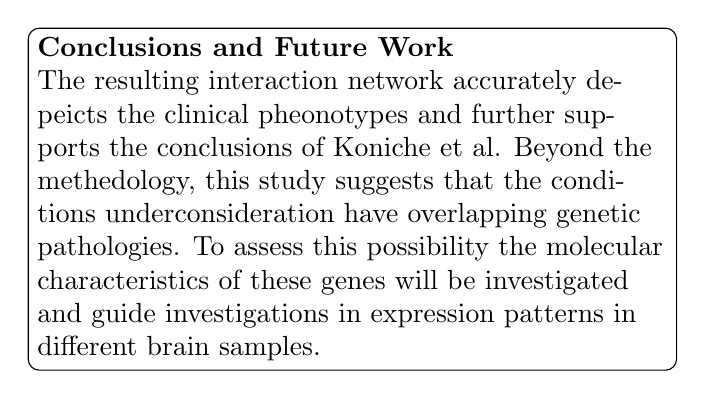
\begin{tikzpicture}
\node (start) [box] {\textbf{Conclusions and Future Work}\\ The resulting interaction network accurately depeicts the clinical pheonotypes and further supports the conclusions of Koniche et al. Beyond the methedology, this study suggests that the conditions underconsideration have overlapping genetic pathologies. To assess this possibility the molecular characteristics of these genes will be investigated and guide investigations in expression patterns in different brain samples.};
\end{tikzpicture} 
\fontsize{12}{12}\selectfont{\textbf{References}}\\
\fontsize{7}{7}\selectfont{1. Kochinke K, Zweier C, Nijhof B, Fenckova M, Cizek P, Honti F, et al. (2016): Systematic Phenomics Analysis Deconvolutes Genes Mutated in Intellectual Disability into Biologically Coherent Modules. Am J Hum Genet. 98:149-164.}\\
\end{multicols*}
\end{document}
